\documentclass{article}
\title{An Investigative Study on the Fabrication of a Projectile Propulsion System} 
\usepackage{graphicx}

\author{Matthew Zhang, Ian May}
\begin{document}
\maketitle

\newpage

\section{Launcher}
{\centering
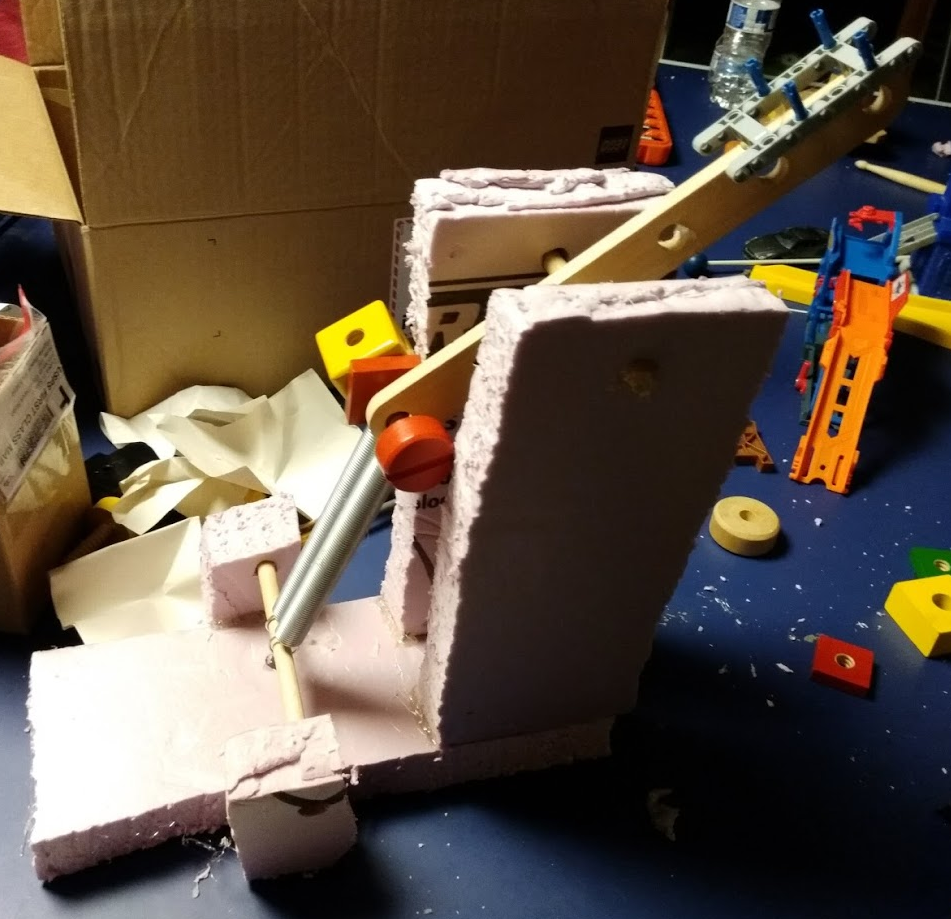
\includegraphics[width=.8\linewidth]{launcher.png}\par}

The launcher features a foam body with 2 extension springs. It employs a simple catapult system, centered around a 1st class lever with the springs on one side, and a ball holder made out of legos on the other side. The lego blocks on the side of the springs serve to stop the launcher at a specific angle to ensure a consistent launch angle. Pulling down the ball side of the lever and releasing it results in the ball being flung from the device.
\newpage

\section{Design Process}
In order to design our launcher, we decided upon a catapult system that would use an 
elastic force to fling the golf ball into the air. We decided upon this design because 
it would be easy to keep the launch angle the same while only adjusting the launch velocity 
by pulling the catapult lever down in order to hit the different squares.


We brought this concept to life using a prototype made out of wooden toy building pieces.
Despite the questionable engineering techniques used to construct it, this first prototype worked relatively well. It was a simple catapult with an extension spring on one side of the lever, and a golf ball holder on the other side. In order to improve upon this concept, we attached a second spring in parallel to double the elastic energy available. Furthermore to optimize the device, we adjusted the location of the pivot along the lever to get the right balance of torque and angular velocity at the ball holder. Lastly we added a triangular brace to prevent the device from collapsing on itself when it was fired. This prototype worked fairly well, and was demonstrated at the check-in. The problems that we identified with this iteration was that it's launch angle was much too shallow, and the tremendous amount of energy provided by the 2 springs was able to launch it far, but the vertical height was not very good. In addition, there was no end-stop to fix a launch angle. 


To further improve our design, we switched to a foam body to provide more flexibility in the building system, as we were being limited by the wooden toys. The new launcher features an endstop mechanism to ensure that it shoots both more vertically and more consistently. In addition, the springs were mounted in a way so that there would be a slight amount of tension at the end of the motion in order to maximize the tension throughout the launch without exceeding the load limit on the spring. Lastly, the angle between the lever and the spring is designed to be closest to 90 degrees near the beginning of the launch in order to maximize torque when the spring tension is highest.


To calibrate the launcher, we shot it at various angles, marked them, and wrote down how far it went horizontally. On test day we plan to plan to figure out the horizontal distance it needs to travel and from there figure out how much we need to pull it back.
\end{document}